
In this section we provide an analysis of the classes of errors observed in
software-defined networks. We base our analysis on conversations with
researchers at Nicira \cite{Nicira}, a startup focused on developing a network operating
system for production SDN deployments \cite{Onix}.

\begin{figure}[t]
    \centering
    \begin{tabular}{ccc}
    \hspace{-3pt}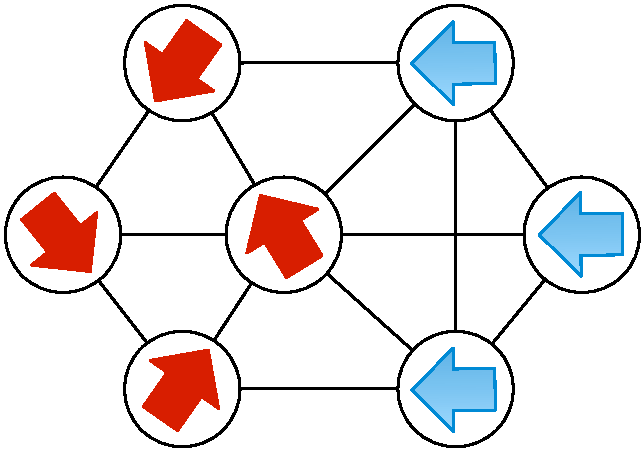
\includegraphics[width=1in]{../diagrams/bugs/loop.pdf}&
    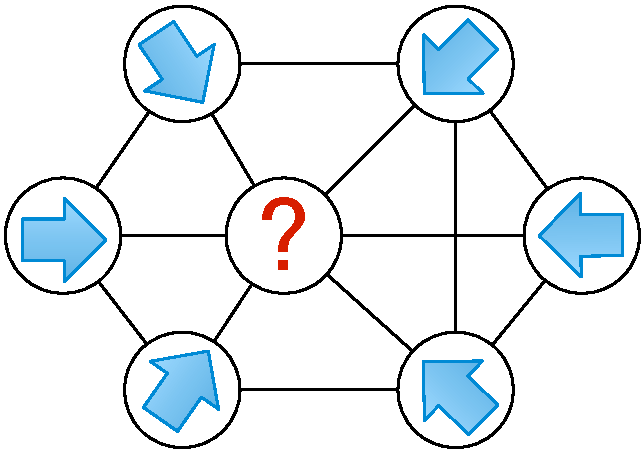
\includegraphics[width=1in]{../diagrams/bugs/dead_end.pdf}&
    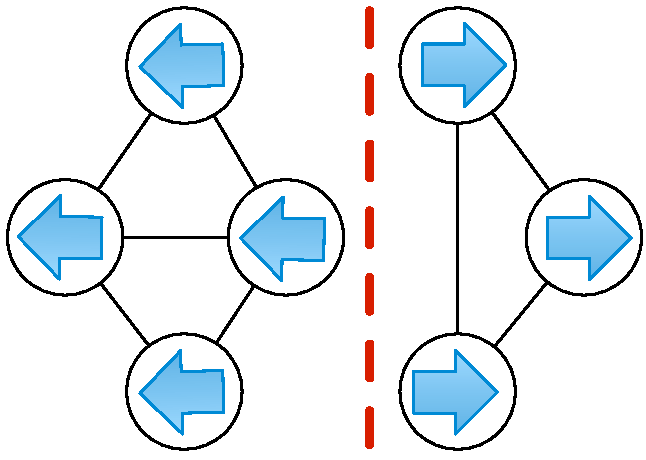
\includegraphics[width=1in]{../diagrams/bugs/partition.pdf}\\
    {\bf (i) Loop}&{\bf (ii) Black Hole}&{\bf (iii) Partition}\\
    \end{tabular}
    \caption[]{\label{fig:loop} Selected classes of physical network errors detectable with static
    checking.\vspace{-10pt}} 
\end{figure}

\colin{Insert diagrams on bugs that we can catch but Anteater can't}

